\chapter{Implementation}
\label{chap:implementation}

\section{Approach}

In a first step we tried to develop a working parser. To test the parser we chose the most complicated logo file in the /logofiles folder. After that one by one we wrote a mapping between the different LOGO Primitives into Java code with the help of the given class LogoPrimitives.

\section{Description of important elements}

\subsection{Comment}

According to the grammar comment lines must be skipped by the parser/translator. We had to add a SKIP expression to our Logo.jj file with a regular expression that will fit to a complete line starting with the \# character.

\begin{center}
SKIP : { <"\#"(\texttildelow["\textbackslash n"])*>}
\end{center}

\subsection{Variables}
At first we were on the wrong track with the variables. We thought that it was necessary to evaluate the Variables and not just translate them, which was a lot of extra work. After rereading the description, we decided to just translate everything into Java without the evaluation part, which was then done quite easily.

\subsection{Loops}

Here an explanation of how we implemented the Repeat keyword, because of it's close link with the REPCOUNT keyword. We chose to map it to a for loop, whose variable is a combination of the prefix i with the current number of indentation. This enables us to use nested repeats and still have a unique counter variable.
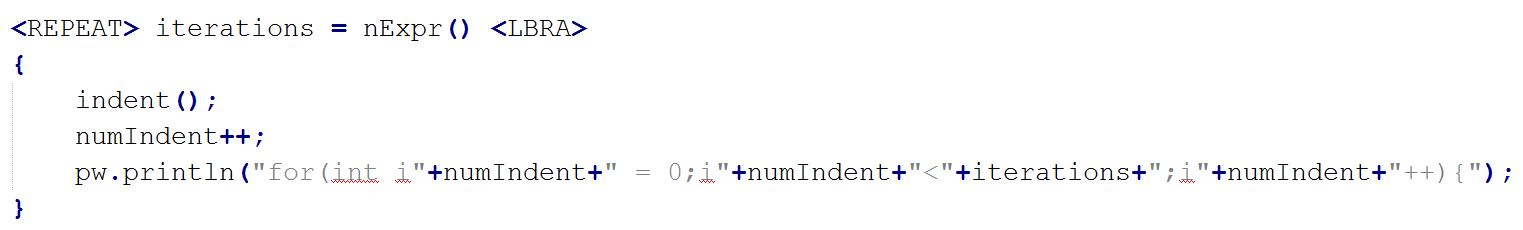
\includegraphics[scale=0.7]{bilder/Repeat.png}\\*
Also it is not a problem if two loops are on the same level of indentation. They will have the same variable name, but because it is in a different scope, the old variable will be hidden by the newly declared.

\subsection{REPCOUNT}
With this chosen approach for loops, the REPCOUNT becomes really easy to implement.\\*
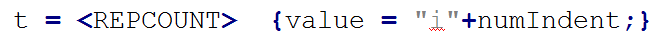
\includegraphics[scale=0.7]{bilder/repcount.png}\\*
We just access the counter variable of the loop that we are in right now, by accessing the indentation that is already remembered by our parser. So even in nested loops, we will always access the right counter variable.

\subsection{Error Warnings}
During the course of our project we encountered different errors, here just the most common ones.
\begin{itemize}
\item Syntaxtic Error: The parser found an syntaxtic error
\item Lexical Error: The lexer has found a bad character sequence
\item Compilation Error of the generated Java File
\end{itemize}

\section{Tests}
\label{sec:tests}
We were running our parser/translator against each one of the files that were given to us for testing purposes. Everything worked just fine. Further we also tested the loops with the same indentation in the file /logofiles/testrep.logo. We also tried looking on the internet for some other examples, but many of them use a version of LOGO which contained Keywords or other grammars (like small lettered identifiers) that could not be understood  by our parser.

\section{Limitations}
\label{sec:limitations}
Our parser is only able to check for syntactic and not semantic errors, although those might be discovered during the compilation process of the generated java program. Apart from that we were able to implement all the features described by the grammar. Obviously the language LOGO itself is quite limited.